\documentclass[11pt] {article}

%%% Preambuła %%%
\usepackage[T1]{fontenc}
\usepackage[polish]{babel}
\usepackage[utf8]{inputenc}
\usepackage{lmodern}
\usepackage[hidelinks]{hyperref}
\usepackage{mathptmx}
\usepackage{float}
\usepackage{graphicx}
\usepackage{amsmath}
\usepackage{xcolor}
\usepackage{listings}
\usepackage{geometry}
\usepackage{tocloft}
\usepackage{subcaption}
\usepackage{indentfirst}
\selectlanguage{polish}
\setlength\parindent{0pt}

\lstset{basicstyle=\ttfamily,
  showstringspaces=false,
  commentstyle=\color{red},
  keywordstyle=\color{blue},
  basicstyle=\ttfamily\footnotesize,
  columns=fullflexible,
  breaklines=true
}

\renewenvironment{abstract}
 {\small
  \begin{center}
  \bfseries \abstractname\vspace{-.5em}\vspace{0pt}
  \end{center}
  \list{}{%
    \setlength{\leftmargin}{5mm}% <---------- CHANGE HERE
    \setlength{\rightmargin}{\leftmargin}%
  }%
  \item\relax}
 {\endlist}

\renewcommand{\cftsecleader}{\cftdotfill{\cftdotsep}} 
\geometry{a4paper, total={170mm,237mm}, left=20mm, top=25mm,}

%%% Strona tytułowa %%%
\title {
	\large Automaty komórkowe \\
    \normalsize Projekt 2: model Isinga
    }

\author {Arkadiusz Kasprzak}
\date{}
	
\begin{document}


%%% Strona tytułowa %%%
\maketitle

%%% Streszczenie %%%
\begin{abstract}
Niniejszy dokument stanowi sprawozdanie z drugiego projektu realizowanego w ramach przedmiotu \textit{Automaty komórkowe}. Tematem projektu było opracowanie interaktywnej aplikacji internetowej implementującej dwuwymiarowy model Isinga, stanowiący matematyczny opis układu oddziałujących spinów. W sprawozdaniu krótko opisana zostanie strona teoretyczna (w tym reguły automatu), następnie omówione zostaną podstawy implementacji oraz testy działania przygotowanej aplikacji - w tym zaobserwowane charakterystyczne zachowania modelu.

\end{abstract}

%%% Spis treści %%%
\tableofcontents

\newpage 

\section{Wstęp}
Celem projektu było stworzenie aplikacji internetowej implementującej dwuwymiarowy model Isinga. Jest to model matematyczny służący do opisu układu spinów \cite{mostowicz}. Opisywanym układem jest więc kwadratowa sieć, której komórki mogą przyjmować jedną z dwóch dyskretnych wartości: $+1$ lub $-1$. Wartość spinu $s$ w danym kroku czasowym determinowana jest na podstawie wartości czterech sąsiednich spinów (otoczenie von Neumanna). W modelu zastosowane zostały periodyczne warunki brzegowe 

\vspace{1.0em}
Model posiada trzy podstawowe parametry: temperatura $T$, tzw. całka wymiany $J$ (określająca charakter oddziaływań spinów: gdy jest dodatnia, to oddziaływania ferromagnetyczne, gdy ujemna - antyferromagnetyczne) oraz wartość zewnętrznego pola magnetycznego $H$. W zależności od wartości temperatury $T$ w modelu stosowana jest jedna z dwóch reguł:
\begin{itemize}
\item dla zerowej temperatury - reguła deterministyczna \cite{malarz, kulakowski} dana zależnością: 
\begin{equation}
s_i(t + 1) = sign \left( \sum_jJ_{ij}s_j + H \right)
\end{equation}
gdzie: $J_{ij}$ - wartość całki wymiany dla spinów $s_i$ oraz $s_j$ (gdy nie są to sąsiednie spiny - wynosi 0), $H$ - zewnętrzne pole magnetyczne. W przypadku, gdy $s_i(t + 1) = 0$, aktualna wartość spinu pozostawiana jest bez zmian.

\item dla niezerowej temperatury ($T > 0$) - algorytm tzw. kąpieli cieplnej \cite{baldyga}. W podejściu tym dla każdego spinu $s_i$ losowana jest liczba rzeczywista $R \in (0, 1)$ oraz obliczona zostaje wartość wyrażenia:
\begin{equation}
r_i(t) = \frac{1}{1 + exp(-2\beta (\sum_{j} J_{ij}s_j + H))}
\end{equation}
gdzie: $\beta = \frac{1}{k_BT}$. Jeśli $R > r_i(t)$, to $s_i(t + 1) = -1$, w przeciwnym razie $s_i(t + 1) = 1$. Reguła ta ma więc charakter probabilistyczny.
\end{itemize}

W obu opisanych przypadkach zaimplementowany algorytm modyfikuje spiny asynchronicznie (w miejscu - bez użycia dodatkowej tablicy zachowującej stan z poprzedniego kroku), od lewego górnego do prawego dolnego rogu sieci. Monitorowanym w ramach modelu parametrem jest tzw. namagnesowanie (magnetyzacja) dane wzorem \cite{wiki}:
\begin{equation}
m = \frac{1}{N} \sum_{i} s_i
\end{equation}
gdzie $N$ - liczba wszystkich spinów w układzie. Wartość tego parametru pozwala określić, która z wartości spinów dominuje w układzie.


\section{Implementacja i opis interfejsu}
Projekt zaimplementowany został w formie prostej aplikacji internetowej (klient) z wykorzystaniem technologii \lstinline{HTML5}, \lstinline{CSS3} oraz języka \lstinline{JavaScript}. Wizualizacja działania automatu (animacja przekształceń sieci) wykonana została z pomocą elementu \lstinline{<canvas>}. Wykres magnetyzacji wykonany został z użyciem biblioteki \lstinline{D3.js} (\lstinline{Data-Driven Documents}) \cite{d3}. Styl strony, poza nielicznymi wyjątkami, oparty został na bibliotece \lstinline{Bootstrap} \cite{bootstrap}. Projekt nie wymaga instalowania żadnych dodatkowych zależności - pliki wykorzystanych bibliotek umieszczone zostały w katalogu \lstinline{resources}.

\vspace{1.0em}

Projekt wykorzystuje funkcjonalności wchodzące w skład standardu \lstinline{ECMAScript 6} - do jego poprawnego działania może być więc konieczne posiadanie stosunkowo nowej wersji przeglądarki. Projekt został przetestowany na dwóch przeglądarkach: Google Chrome (wersja 80.0.3987.132) oraz Firefox (wersja 73.0.1).


\begin{figure}[H]
\centering
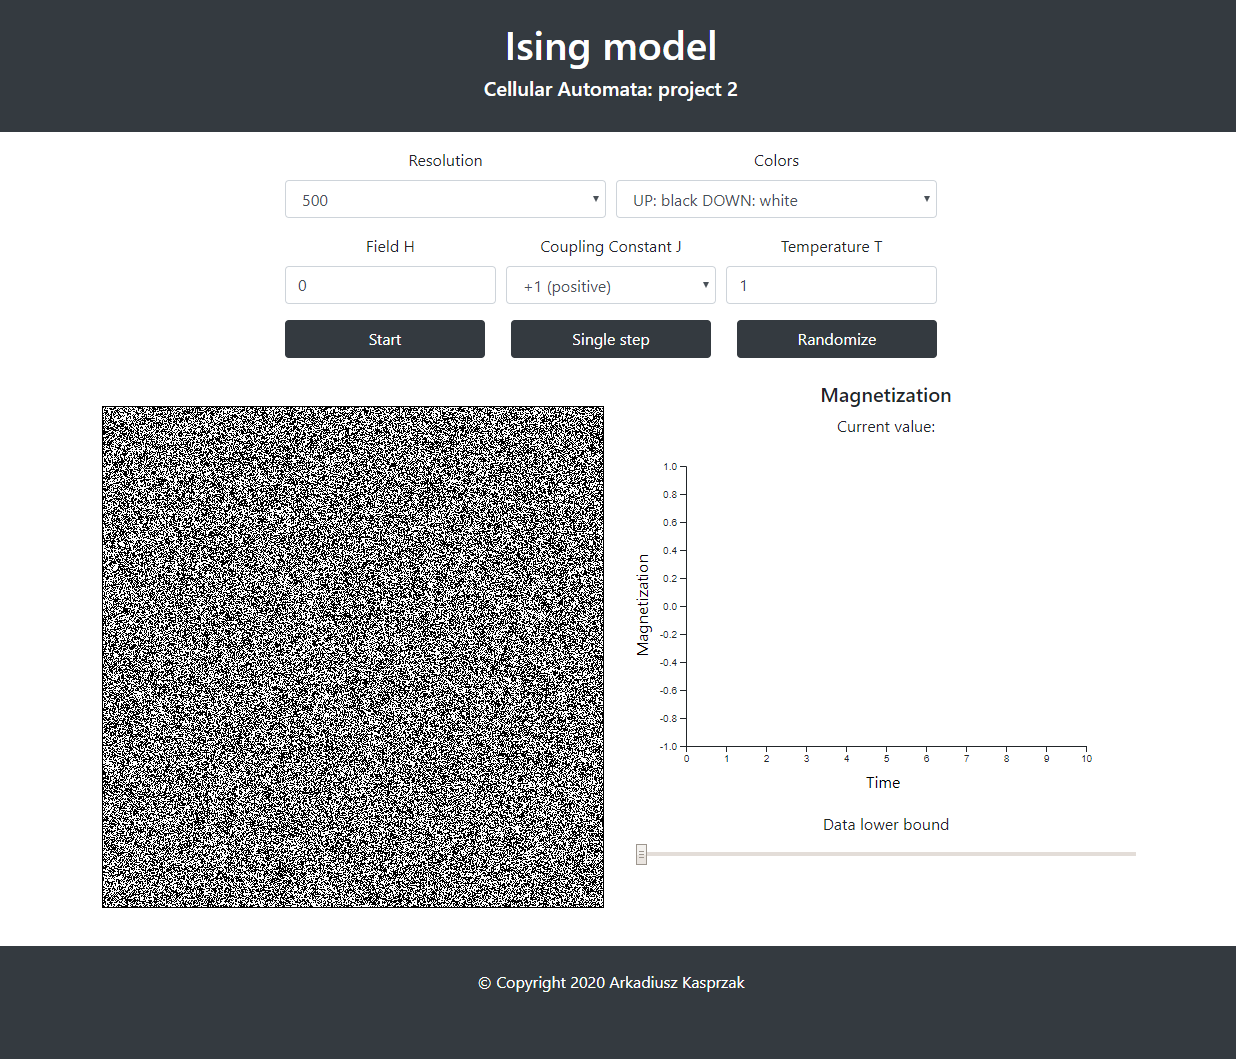
\includegraphics[width=\textwidth]{res/interface.png}
\caption{Interfejs aplikacji. W górnej części widoczne menu pozwalające na konfigurację modelu. Poniżej, po lewej stronie znajduje się obszar odpowiedzialny za wizualizację przebiegu symulacji. Na prawo od niego widoczny jest natomiast wykres magnetyzacji od czasu.}
\label{fig:interface}
\end{figure}

Rysunek \ref{fig:interface} przedstawia interfejs przygotowanej aplikacji. Składa się on z trzech podstawowych elementów: 
\begin{itemize}
\item menu - znajduje się w górnej części interfejsu i pozwala użytkownikowi na konfigurację modelu. Udostępnione parametry to: rozdzielczość siatki, na której wykonywana jest symulacja, konfiguracja kolorów, wartość zewnętrznego pola $H$, wartość stałej oddziaływania (całki wymiany) $J$ oraz wartość temperatury $T$. Menu zawiera również trzy przyciski odpowiedzialne za: rozpoczęcie/zatrzymanie symulacji, wykonanie pojedynczego kroku w symulacji oraz wygenerowanie nowego, losowego stanu początkowego. Niektóre z opisanych funkcjonalności (np. zmiana rozdzielczości) nie są dostępne w czasie działania modelu.

\item animacja - kwadratowy obszar, w którym wyświetlana jest animacja obrazująca aktualny stan modelu. Prędkość animacji jest automatycznie dobierana zgodnie z częstotliwością odświeżania ekranu (typowo około 30-60 klatek na sekundę).

\item wykres namagnesowania w funkcji czasu - znajduje się na prawo od obszaru animacji. Nad wykresem wyświetlana jest aktualna wartość magnetyzacji. Domyślnie na wykresie prezentowana jest magnetyzacja dla maksymalnie 250 ostatnich kroków czasowych (jest to podyktowane kwestiami związanymi z wydajnością). Po zatrzymaniu symulacji możliwy jest natomiast wybór minimalnej wartości wyświetlanej na osi czasu (za pomocą suwaka znajdującego się pod wykresem).
\end{itemize}


\section{Testy działania}
W ramach prac nad projektem przeprowadzone zostały testy jego działania dla różnych wartości parametrów wejściowych. Niniejsze sprawozdanie zawiera rezultaty kilku wybranych przez autora testów. W celu zmniejszenia czasu trwania testów wykorzystane zostały modele o rozdzielczości 250 oraz 100.

\vspace{1.0em} 
Pierwszy z testów zakładał zbadanie wpływu temperatury na zachowanie modelu. Rysunek \ref{fig:T} przedstawia wyniki uzyskane dla czterech przykładowych wartości temperatury. Całka wymiany była w tym przypadku dodatnia, a zewnętrzne pole magnetyczne wyłączone. W każdym przypadku przedstawiony został zarówno stan układu w wybranym kroku czasowym, jak i wykres magnetyzacji opisujący jej zmiany od momentu rozpoczęcia symulacji.

\begin{figure}[H]
\centering
\begin{subfigure}{.48\textwidth}
  \centering
  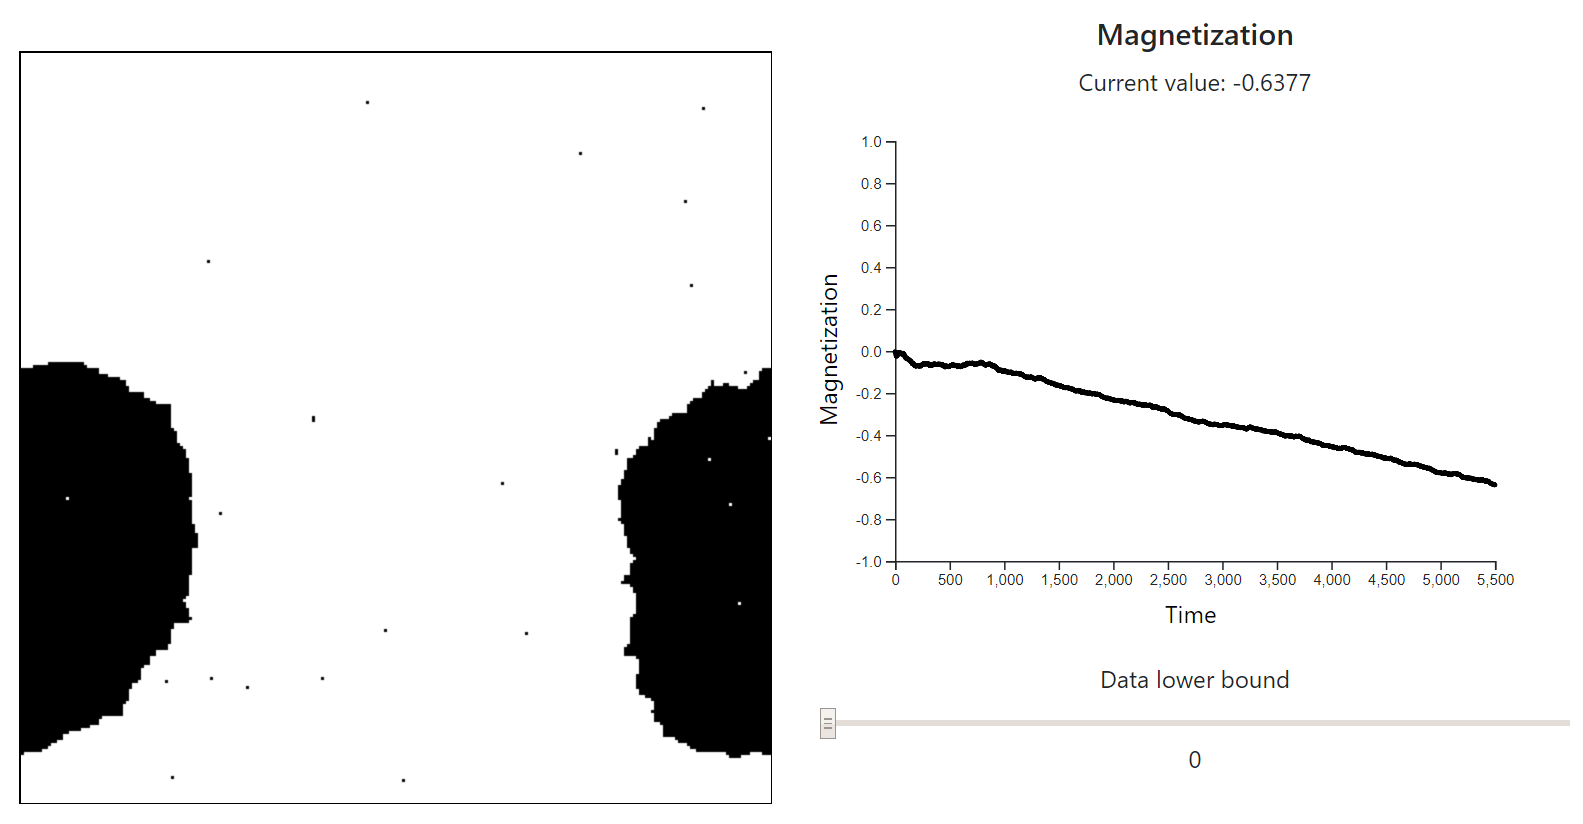
\includegraphics[width=0.9\linewidth]{res/T_1.png}
  \caption{Stałe $T = 1.0$ - przypadek pierwszy}
  \label{fig:T1}
\end{subfigure}
\begin{subfigure}{.48\textwidth}
  \centering
  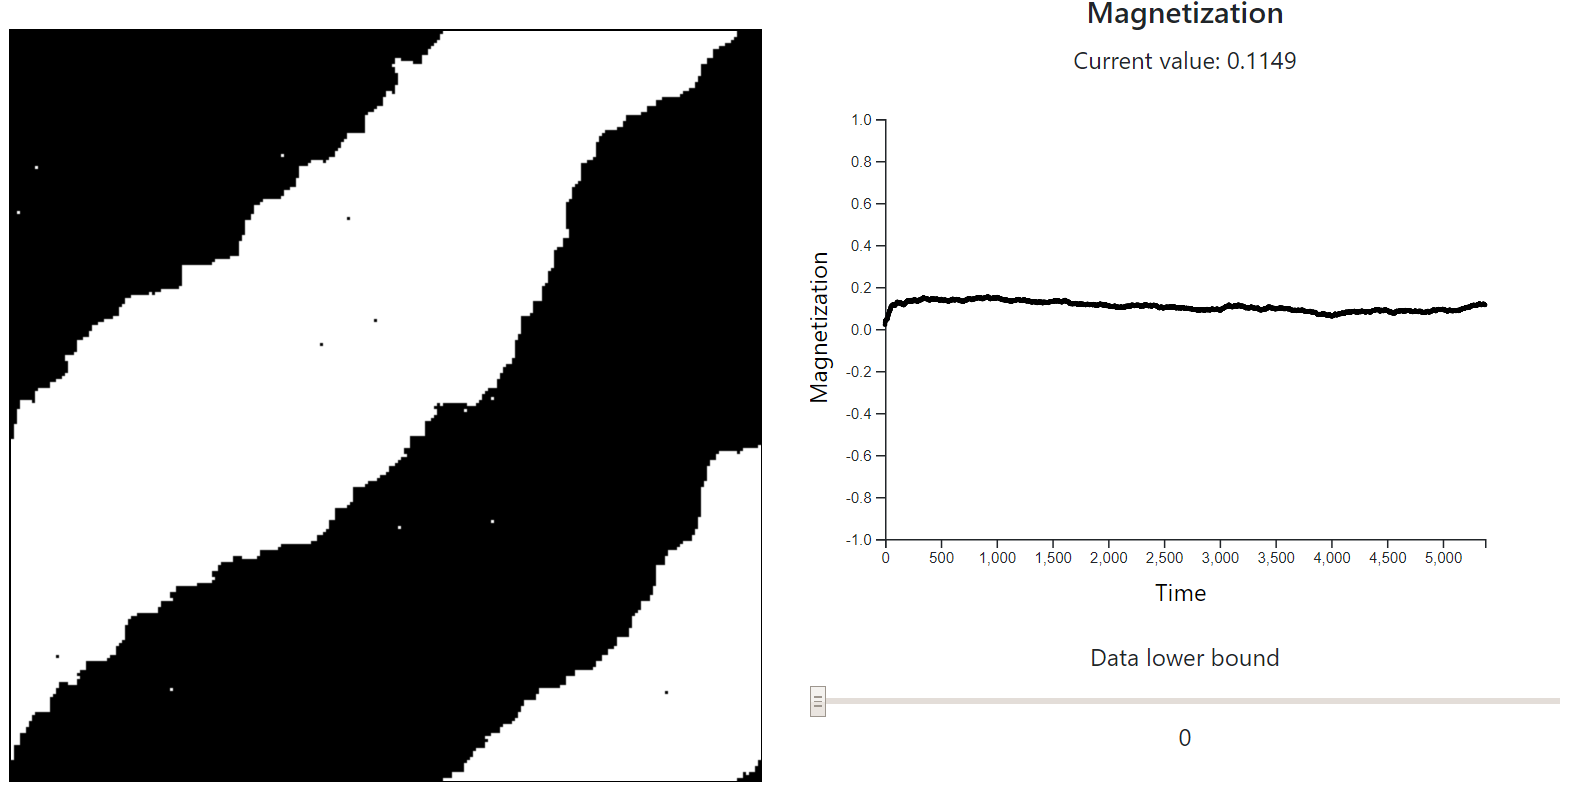
\includegraphics[width=0.9\linewidth]{res/T_1_2.png}
  \caption{Stałe $T = 1.0$ - przypadek drugi}
  \label{fig:T12}
\end{subfigure}
\begin{subfigure}{.48\textwidth}
  \centering
  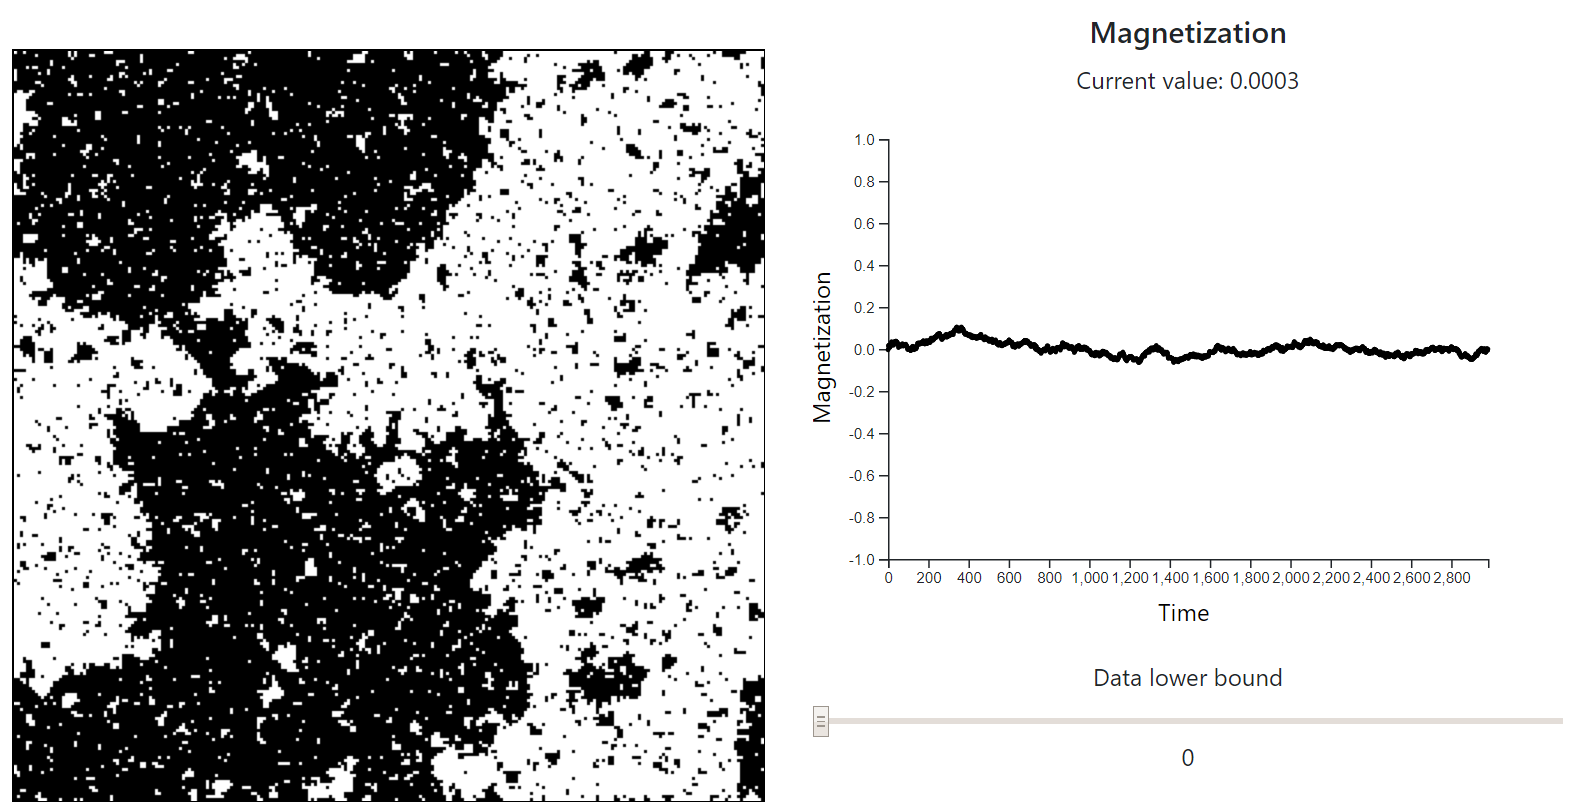
\includegraphics[width=0.9\linewidth]{res/T_2_2.png}
  \caption{Stałe $T = 2.2$}
  \label{fig:T2}
\end{subfigure}
\begin{subfigure}{.48\textwidth}
  \centering
  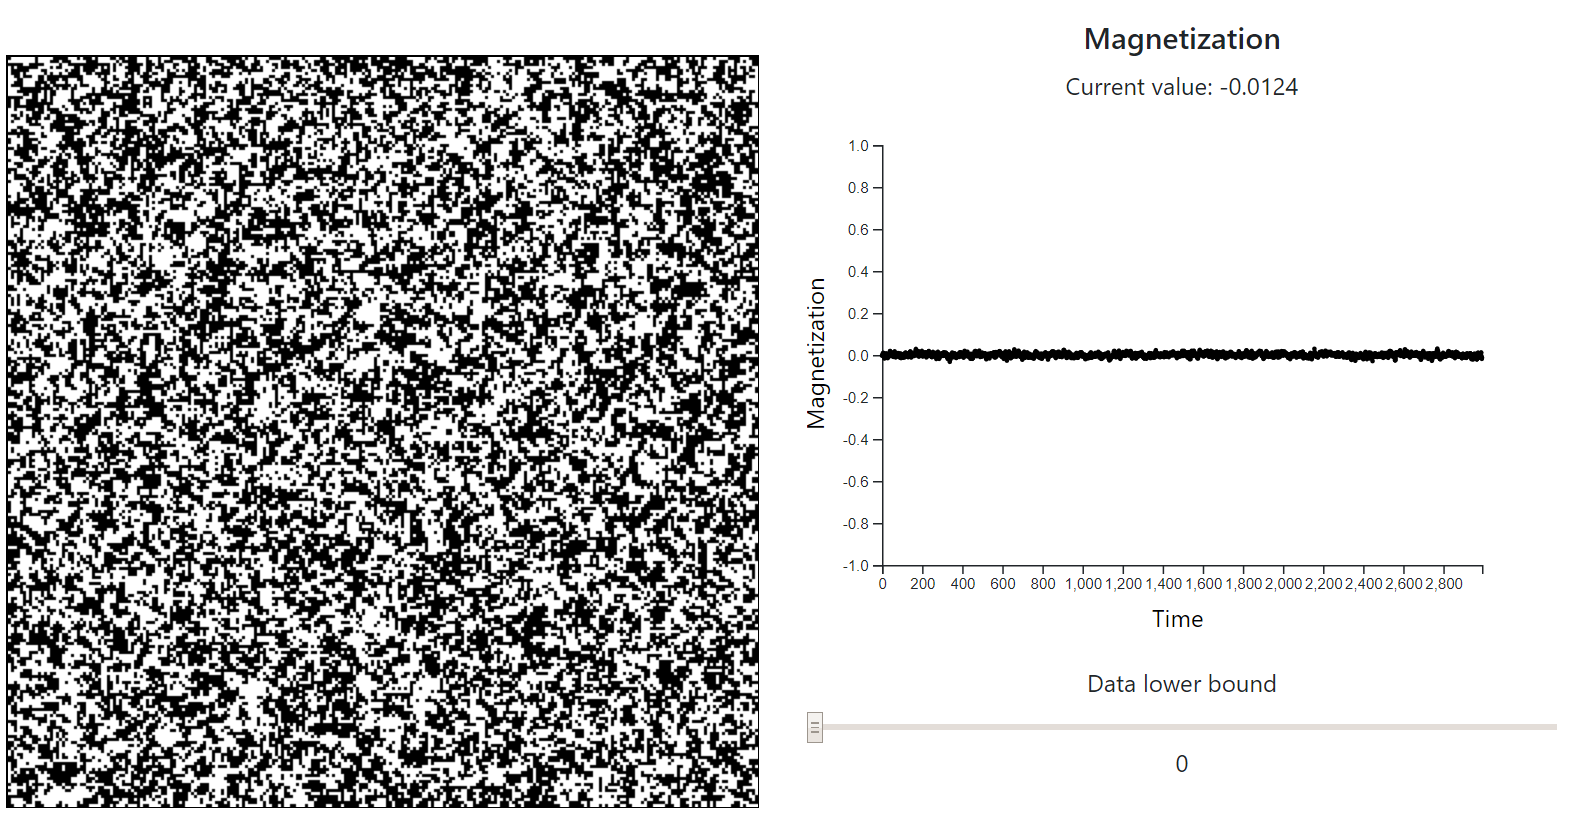
\includegraphics[width=0.9\linewidth]{res/T_4.png}
  \caption{Stałe $T = 4.0$}
  \label{fig:T4}
\end{subfigure}
\begin{subfigure}{.48\textwidth}
  \centering
  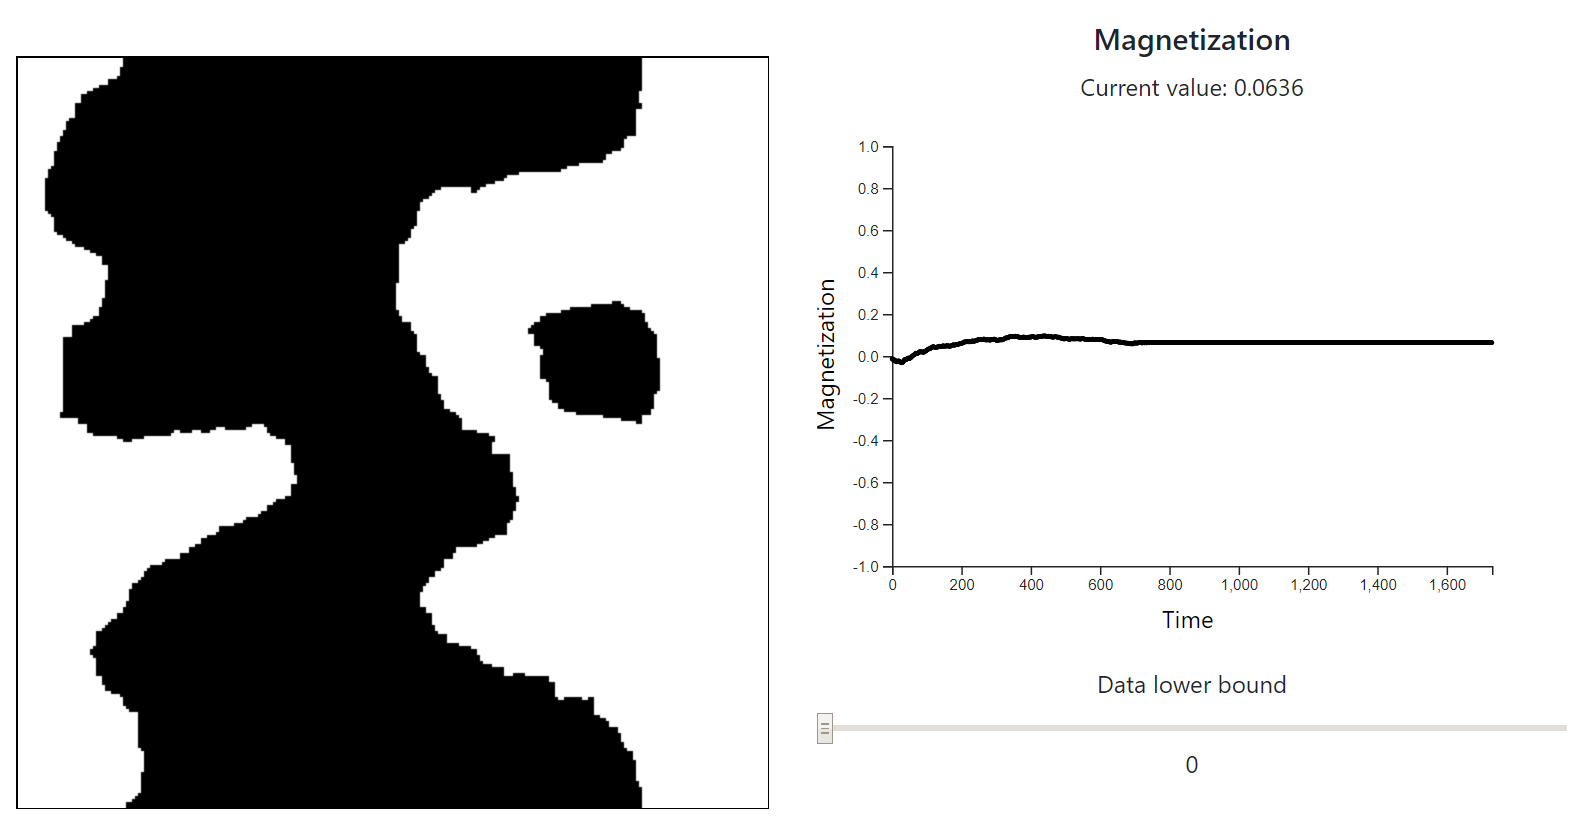
\includegraphics[width=0.9\linewidth]{res/T_0.png}
  \caption{$T = 1.0$ początkowo, następnie przejście do $T = 0.0$}
  \label{fig:T0}
\end{subfigure}
\caption{Zachowanie układu dla $J = +1$, $H = 0$ i różnych wartości temperatury $T$.}
\label{fig:T}
\end{figure}

Jak wynika z załączonych wyników zachowanie układu zmienia się znacząco wraz ze zmianą temperatury. Dla niewielkiej, ale niezerowej wartości ($T = 1.0$) układ przechodzi powolną ewolucję (rys. \ref{fig:T1}). W przypadku przedstawionym na rysunku zdaje się powoli (symulacja zatrzymana w tym przypadku po około 5500 krokach czasowych) dążyć do sytuacji w której większość spinów skierowana będzie w tym samym kierunku (w dół). Wielokrotne powtórzenie takiego badania potrafi jednak przynieść odmienne wyniki - w niektórych przypadkach układ nawet po tak długim czasie pozostawał w okolicach zerowego namagnesowania (rys \ref{fig:T12} - charakterystyczny wzór ,,pasów''). Zdarzało się również, że dotarcie do jednej ze skrajnych wartości magnetyzacji przebiegało znacznie szybciej. Dla wyższej temperatury ($T = 2.2$) uzyskane wyniki różniły się pod kilkoma względami. Temperaturę w tym przypadku traktować można jak wprowadzenie do układu szumu - co jest wyraźnie widoczne na rys. \ref{fig:T2}. Losowe zmiany wartości spinów spowodowane temperaturą powodują powstanie wielu niewielkich ,,plam'' - obszarów o odmiennym od otoczenia spinie. Wykres magnetyzacji również ilustruje to zjawisko - widoczne są na nim fluktuacje. Podobnie jak wcześniej wielokrotnie uruchomienie symulacji może prowadzić do innych wyników jeśli chodzi o osiągane wartości namagnesowania. Przypominające szum zachowanie układu potęguje się wraz ze wzrostem temperatury - dla $T = 4.0$ (rys. \ref{fig:T4}) wartości spinów zdają się być w zupełności losowe. Wartość namagnesowania fluktuuje w tym przypadku wokół zera. Inaczej wygląda ewolucja modelu w sytuacji, gdy $T = 0$. W przypadku przedstawionym na rysunku \ref{fig:T0} temperatura została po krótkim czasie trwania symulacji przełączona z $1.0$ na właśnie $0.0$, co spowodowało zatrzymanie się automatu - jego stan przestał ulegać zmianom, a co za tym idzie namagnesowanie pozostało stałe. Ponieważ brak jest jakichkolwiek zmian lub oscylacji, mamy w tym przypadku do czynienia z automatem komórkowym klasy I (według klasyfikacji Wolframa \cite{malarz, kulakowski}).

\vspace{1.0em} 
Podobne badania przeprowadzone zostały dla ujemnej wartości całki wymiany ($J = -1$) - wyniki przedstawione zostały na rysunku \ref{fig:TJN}. Jeśli chodzi o wpływ temperatury to układ zachowuje się w tym przypadku tak samo jak poprzednio - zwiększenie temperatury wprowadza szum, zerowa temperatura powoduje, że zmiany w stanie automatu nie zachodzą. Inaczej natomiast wygląda sam układ spinów. Dla ujemnej całki wymiany preferowane jest naprzemienne występowanie wartości spinów, tzn: $+1, -1, +1, ...$ (co prowadzi co niemal zerowej wartości namagnesowania), natomiast dla jej dodatniej wartości układ dążył do sytuacji, w której wszystkie spiny miały takie same wartości - preferowane więc były ustawienia $+1, +1, +1, ...$ lub $-1, -1, -1, ...$.

\begin{figure}[H]
\begin{subfigure}{.5\textwidth}
  \centering
  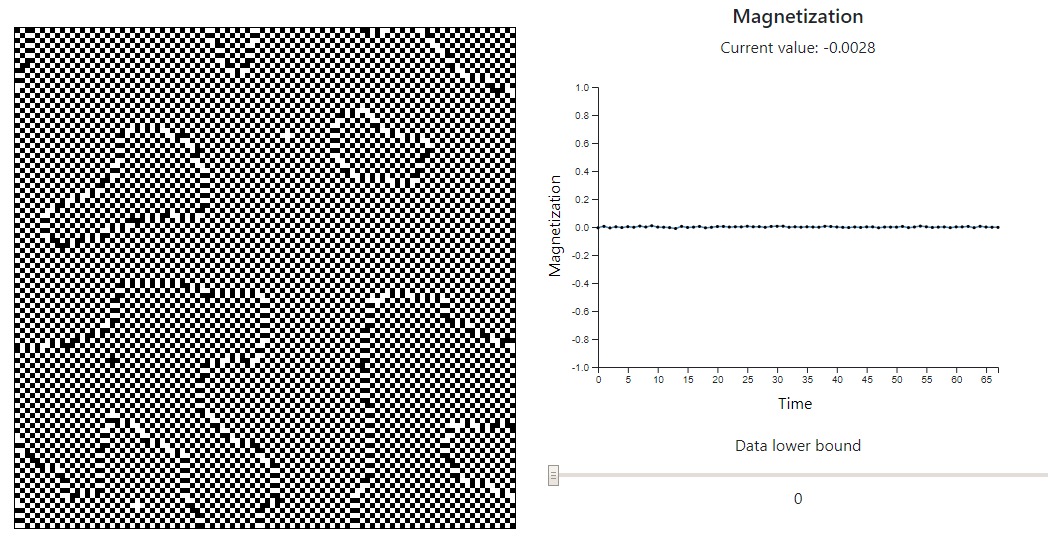
\includegraphics[width=0.9\linewidth]{res/T_1_negative.png}
  \caption{Stałe $T = 1.0$}
  \label{fig:TJN1}
\end{subfigure}
\begin{subfigure}{.5\textwidth}
  \centering
  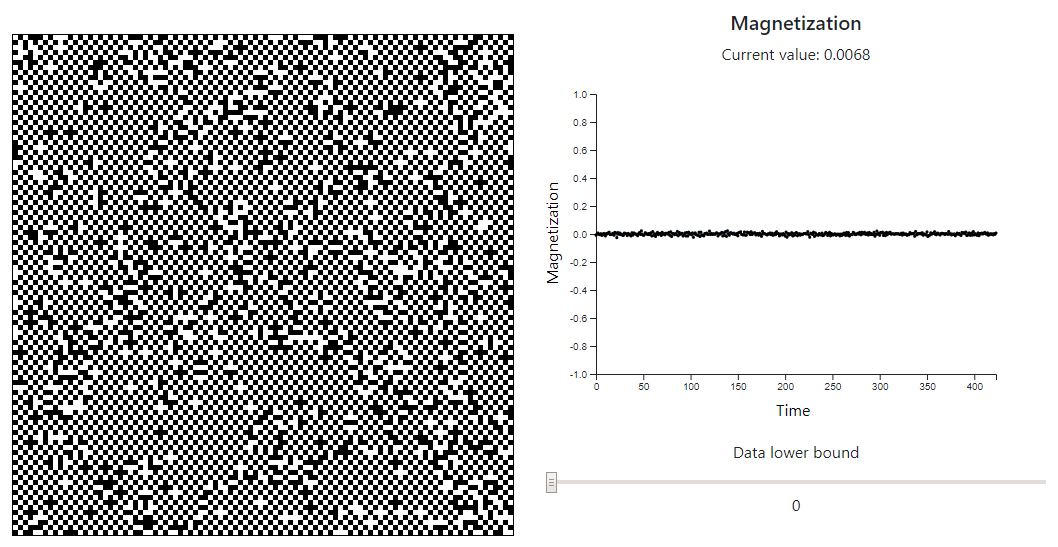
\includegraphics[width=0.9\linewidth]{res/T_2_2_negative.png}
  \caption{Stałe $T = 2.2$}
  \label{fig:TJN2}
\end{subfigure}
\begin{subfigure}{.5\textwidth}
  \centering
  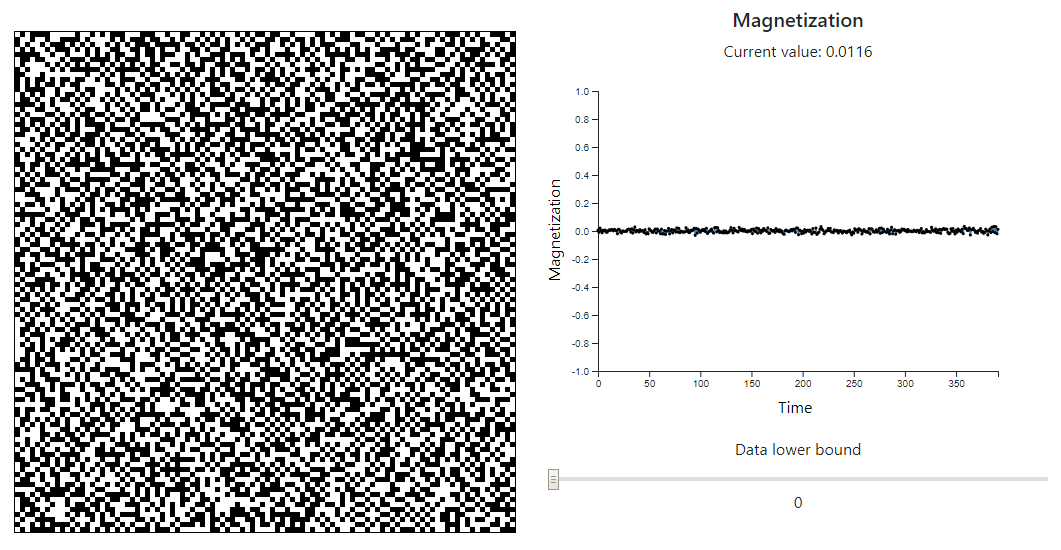
\includegraphics[width=0.9\linewidth]{res/T_4_negative.png}
  \caption{Stałe $T = 4.0$}
  \label{fig:TJN4}
\end{subfigure}
\begin{subfigure}{.5\textwidth}
  \centering
  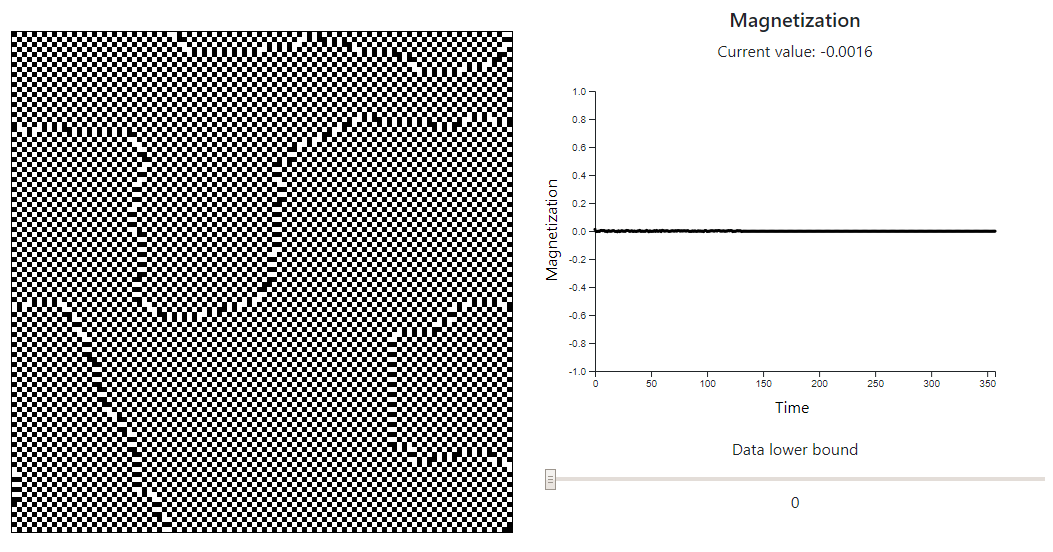
\includegraphics[width=0.9\linewidth]{res/T_0_negative.png}
  \caption{$T = 1.0$ początkowo, następnie $T = 0.0$}
  \label{fig:TJN0}
\end{subfigure}
\caption{Zachowanie układu dla $J = -1$, $H = 0$ i różnych wartości temperatury $T$.}
\label{fig:TJN}
\end{figure}

\newpage
Wprowadzenie zewnętrznego pola magnetycznego o nawet niewielkiej wartości ma znaczny wpływ na zachowanie układu, co obrazuje rysunek \ref{fig:H}. Dla sieci o wymiarach $250 \times 250$ komórek i całki wymiany o wartości dodatniej zmiana wartości pola na $H = 0.1$ prowadzi do bardzo szybkiej ewolucji układu w stronę wartości magnetyzacji równej $1.0$ (niemal każdy spin skierowany jest w górę). Analogicznie dla zmiany wartości pola na $H = -0.1$ układ zaczyna szybko dążyć do ustawienia, w którym wszystkie spiny skierowane są w dół. Dla ujemnych wartości całki wymiany proces ten przebieg wolniej, dla $H=3.0$ przypomina to, podobnie jak duża wartość temperatury, rodzaj szumu (rys. \ref{fig:HJneg}) . W tym przypadku zmiany mają charakter skokowy, dla odpowiednio dużej wartości $H$ pozwalają jednak osiągać wartości magnetyzacji zbliżone skrajnym.

\begin{figure}[H]
\begin{subfigure}{.5\textwidth}
  \centering
  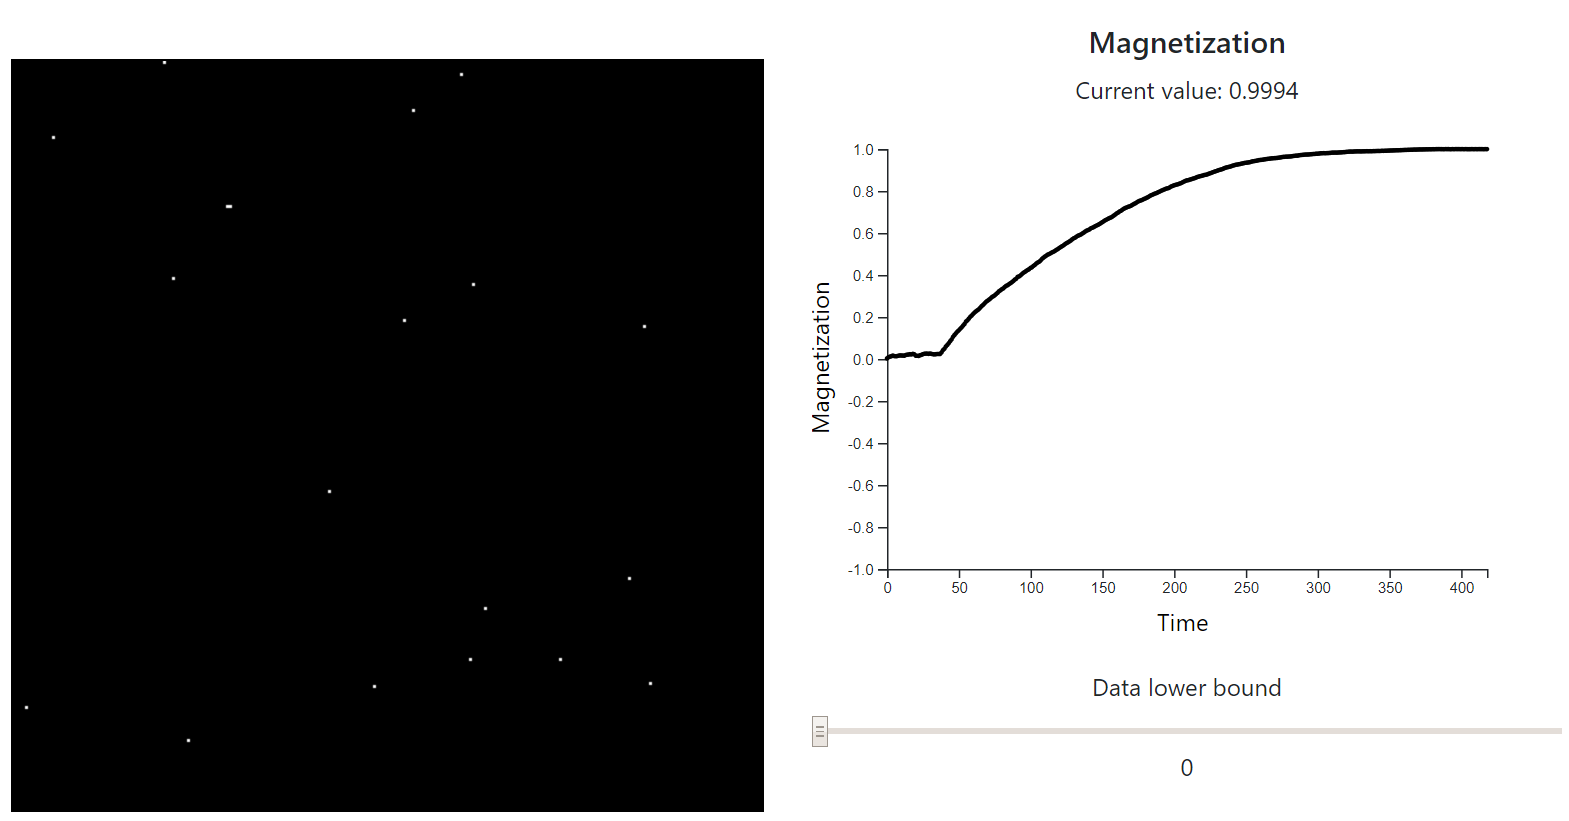
\includegraphics[width=0.9\linewidth]{res/Hplus.png}
  \caption{Zewnętrzne pole $H = 0.1$}
  \label{fig:H1}
\end{subfigure}
\begin{subfigure}{.5\textwidth}
  \centering
  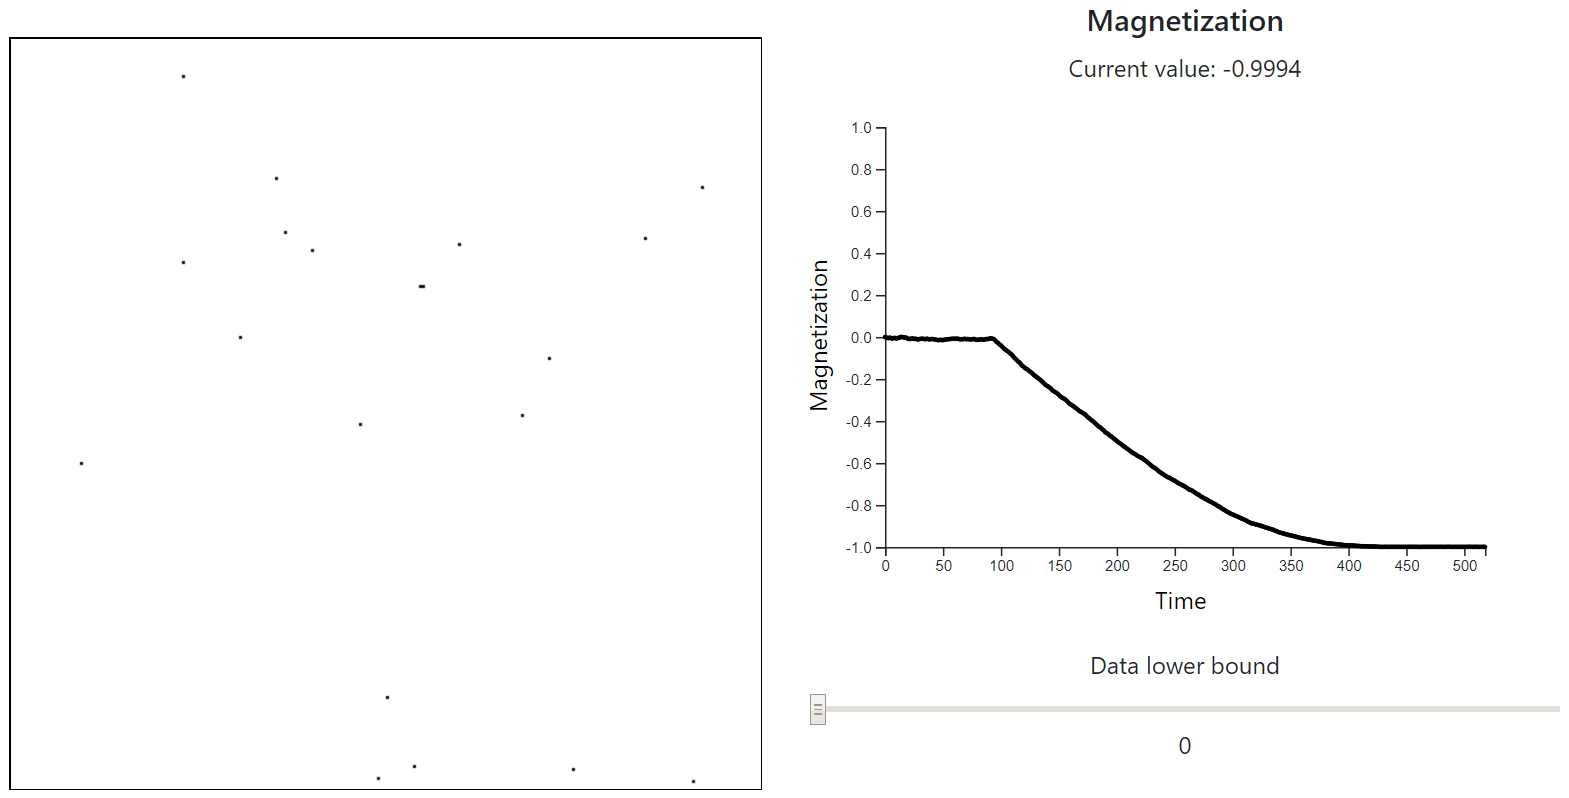
\includegraphics[width=0.9\linewidth]{res/Hminus.png}
  \caption{Zewnętrzne pole $H = -0.1$}
  \label{fig:H2}
\end{subfigure}
\caption{Zachowanie układu dla $J = +1$, $T = 1.0$ oraz różnych wartości pola $H$.}
\label{fig:H}
\end{figure}

\begin{figure}[H]
\centering
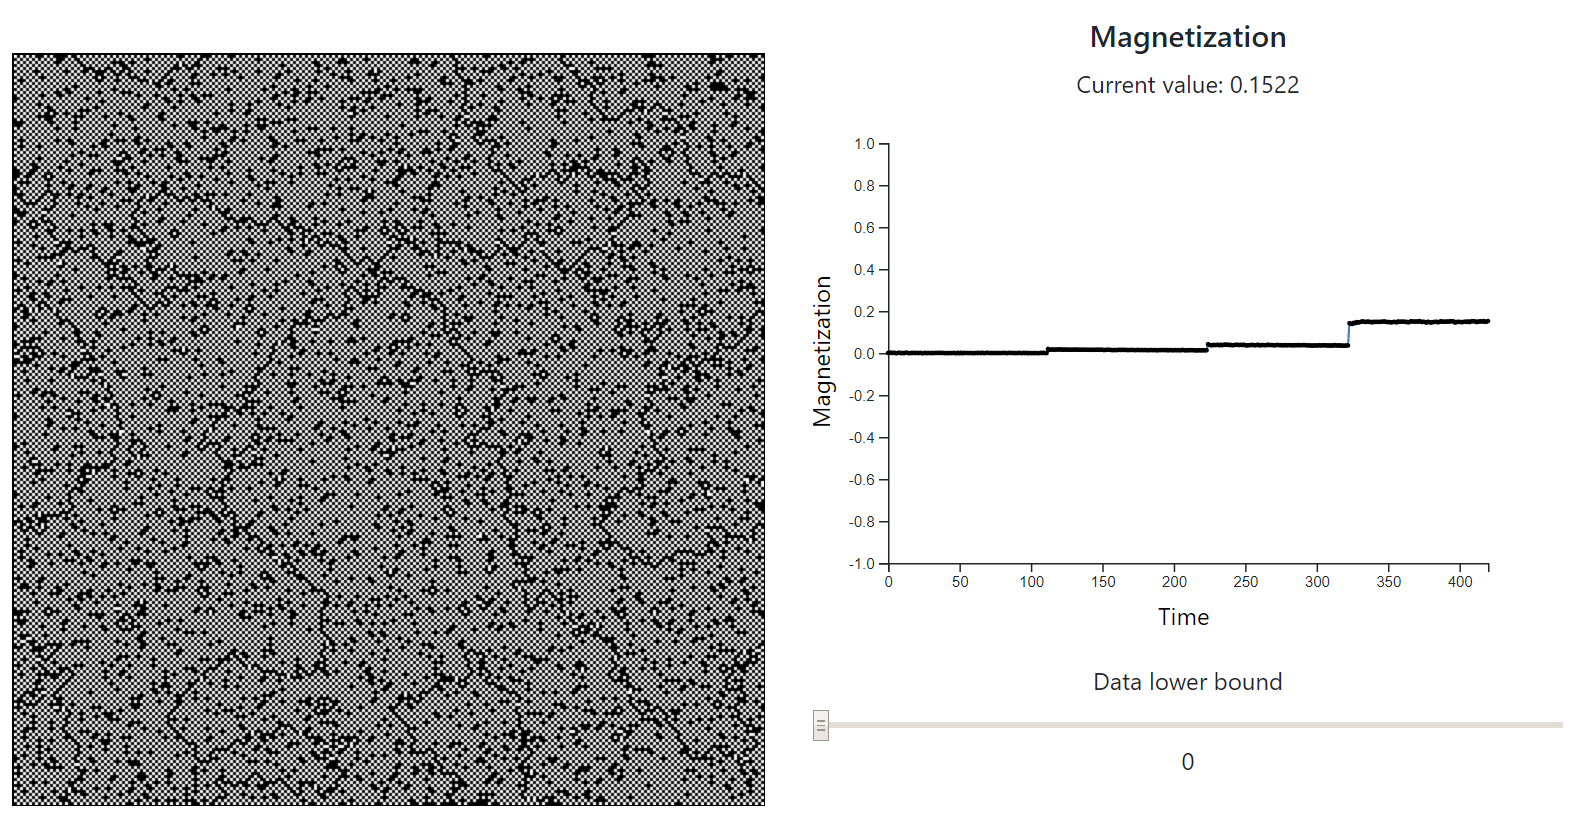
\includegraphics[width=0.9\linewidth]{res/Hplus2.png}
\caption{Zachowanie układu dla $J = -1$, $T = 1.0$ i zwiększania wartości pola $H$.}
\label{fig:HJneg}
\end{figure}

Ciekawym przypadkiem jest zmiana wartości pola, gdy do czynienia mamy z dużą wartością temperatury (np. $T = 4.0$). Dla zerowego pola taki przypadek oznaczał oscylację namagnesowania wokół wartości $0.0$. Rysunek \ref{fig:HTlarge} przedstawia wynik uzyskany dla wysokiej temperatury i skokowej zmiany wartości pola. W tym przypadku wartość magnetyzacji również maleje skokowo - gdy pole pozostaje stałe, oscyluje wokół nowej wartości.

\begin{figure}[H]
\centering
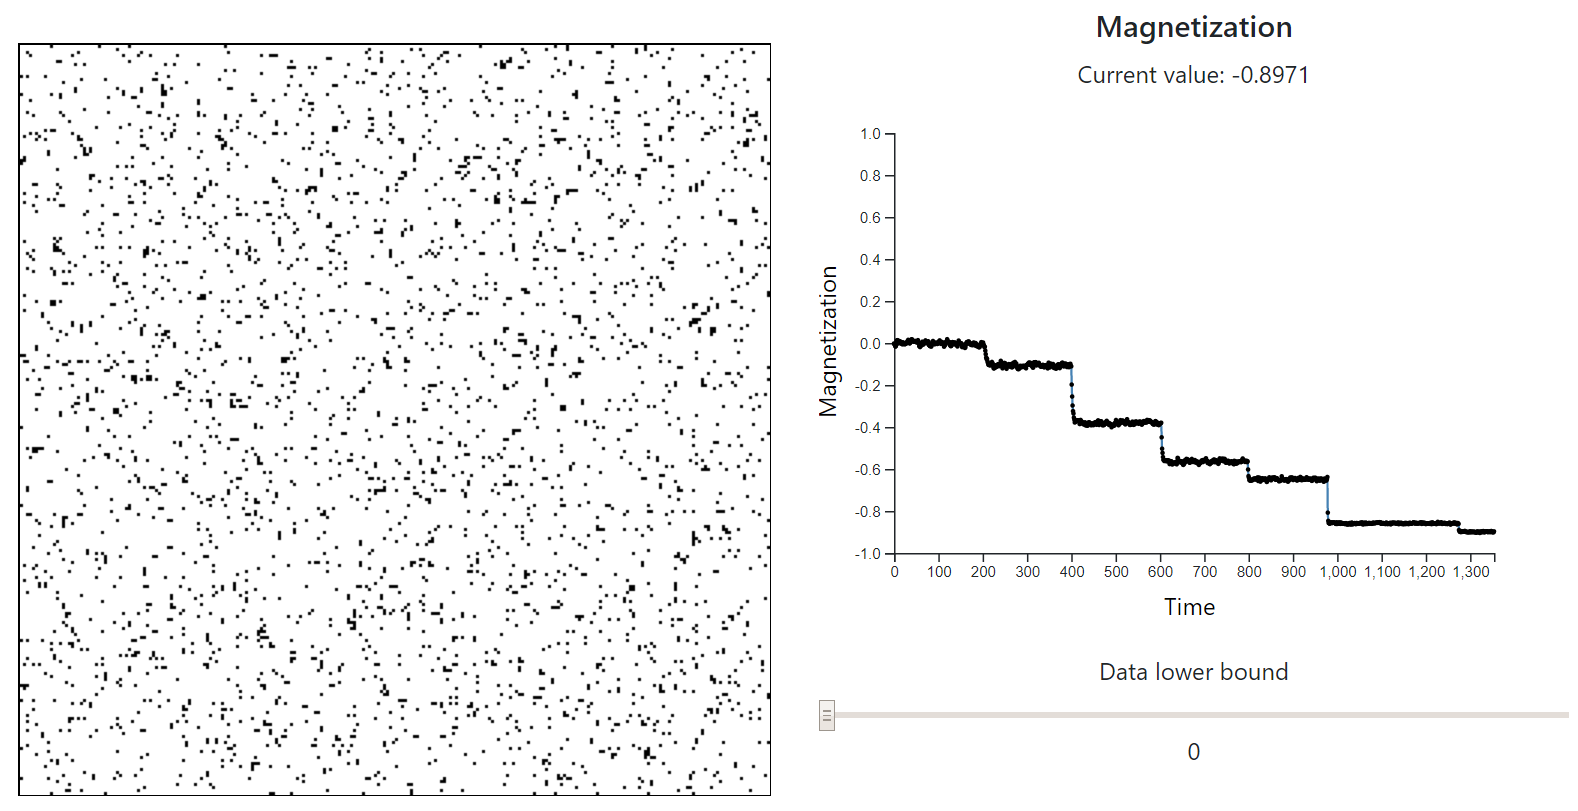
\includegraphics[width=0.9\linewidth]{res/HnegT4.png}
\caption{Zachowanie układu dla $J = +1$, $T = 4.0$ i skokowego zmniejszania wartości pola $H$ aż do $-2.5$.}
\label{fig:HTlarge}
\end{figure}

\section{Wnioski}
\begin{itemize}
\item udało się stworzyć poprawnie działającą implementację dwuwymiarowego modelu Isinga wykorzystującą algorytm kąpieli cieplnej w sytuacji, gdy $T > 0$, oraz regułę deterministyczną, gdy $T = 0$
\item dla układów o dużej rozdzielczości (np. $500 \times 500$ komórek) ewolucja przebieg bardzo powoli
\item dla niewielkiej temperatury i dodatniej wartości całki wymiany układ dążył do stanu, w którym sąsiednie spiny miały takie same wartości
\item w niektórych przypadkach miała miejsce sytuacja, w której układ pomimo upływu długiego czasu pozostawał w stanie, w którym wartość magnetyzacji była bliska 0.0
\item dla niewielkiej temperatury oraz ujemnej wartości całki wymiany układ zwykle dążył do stanu, w którym sąsiednie spiny miały przeciwne wartości
\item temperatura pełni w przypadku modelu Isinga funkcję podobną do szumu
\item zewnętrzne pole magnetyczne ukierunkowuje ewolucję układu w stronę jednej ze skrajnych wartości magnetyzacji - w przypadku dodatniej wartości całki wymiany ewolucja ta przebiega szybko i w sposób ciągły, natomiast dla ujemnej wartości całki ma charakter skokowy - zmiany magnetyzacji następują wraz ze zmianami wartości pola
\end{itemize}


\newpage

\begin{thebibliography}{9}

\bibitem{malarz}
  dr hab. inż. Krzysztof Malarz, prof. AGH,
  \emph{wykład prowadzony w ramach przedmiotu Automaty komórkowe}

\bibitem{kulakowski}
  Krzysztof Kułakowski,
  \emph{Automaty komórkowe}

\bibitem{mostowicz}
  Jacek Mostowicz, 
  \emph{Wykładniki krytyczne modelu Isinga na sieciach (3, 3, 3, 3, 6) i (3, 4, 6, 4) Archimedesa},
  \url{http://mostowicz.pl/doki/mgr_wyk_kryt_m_i.pdf} (dostęp: 02.05.2020)


\bibitem{baldyga}
  Tomasz Bałdyga,
  \emph{Wyznaczenie temperatury krytycznej modelu Isinga na sieciach o rozkładzie potęgowym},
  \url{http://efizyka.if.pw.edu.pl/twiki/pub/FSiT/ProjektyQuiz/TomaszBaldyga.pdf} (dostęp: 02.05.2020)

\bibitem{wiki}
  Wikipedia, The Free Encyclopedia,
  \emph{Ising model},
  \url{https://en.wikipedia.org/wiki/Ising_model} (dostęp: 02.05.2020)

\bibitem{miszczak}
  Jarosław Miszczak,
  \emph{Obliczenia inspirowane Naturą. Wykład 03 - Zastosowanie automatów komórkowych},
  \url{https://iitis.pl/~miszczak/files/natcomp/03_zastosowania_automatow.pdf} (dostęp: 02.05.2020)

\bibitem{carlon}
  E. Carlon,
  \emph{Advanced Monte Carlo Methods},
  \url{http://itf.fys.kuleuven.be/~enrico/Teaching/monte_carlo_2012.pdf} (dostęp: 02.05.2020)

\bibitem{d3}
  Strona internetowa biblioteki \lstinline{D3.js},
  \url{https://d3js.org/} (dostęp: 02.05.2020)

\bibitem{bootstrap}
  Strona internetowe biblioteki \lstinline{Bootstrap},
  \url{https://getbootstrap.com/} (dostęp: 02.05.2020)


\end{thebibliography}

\end{document}